\subsection{What generates spatial variation}\label{sec:variation}
The background-treatment comparison varies the background treatment. Eight largest published OD demands, all incident to node 10, change jointly from $0.2$ to $1.6$ times their base values; every study OD has ten fixed paths. The no-background, frozen-background and responsive-background assignments use zero background, frozen background link flows, and fixed background demands with endogenous rerouting, respectively. The responsive-background assignment assigns all 528 positive demands (full protocols in Appendix~\ref{supp:fields}).
Uniform weights provide a compatible control. The active-link outcome $T(F)=F_{10\to16}$ preserves the $(10,16)$ direction but permits a response-dependent scale; TSTT produces internal imbalance. Figure~\ref{fig:respfield} illustrates the three patterns on the same realized response: compatible weights give one common account on every boundary, the directional outcome balances along the OD but scales with the response, and TSTT weights generate genuine spatial structure. For its seed-zero TSTT response, expanding $\{10\}$ to $\{10,17\}$ lowers the account from $5.77\times10^4$ to $4.34\times10^4$, approximately $92\%$ of the unrestricted spread. The direct-SUE decrease is $24.80\%$ of its own origin-cut account (Appendix~\ref{supp:accuracy}). Both sides of these regions are connected. Free-flow weights explain $84.7\%$ of the node-17 imbalance: all incident links have free-flow time 2 except $10\leftrightarrow17$ with time 8, giving $[B\operatorname{diag}(t_0)G_j]_{17}=6(G_{10\to17,j}-G_{17\to10,j})$.
\begin{figure}[pos=t]
\centering
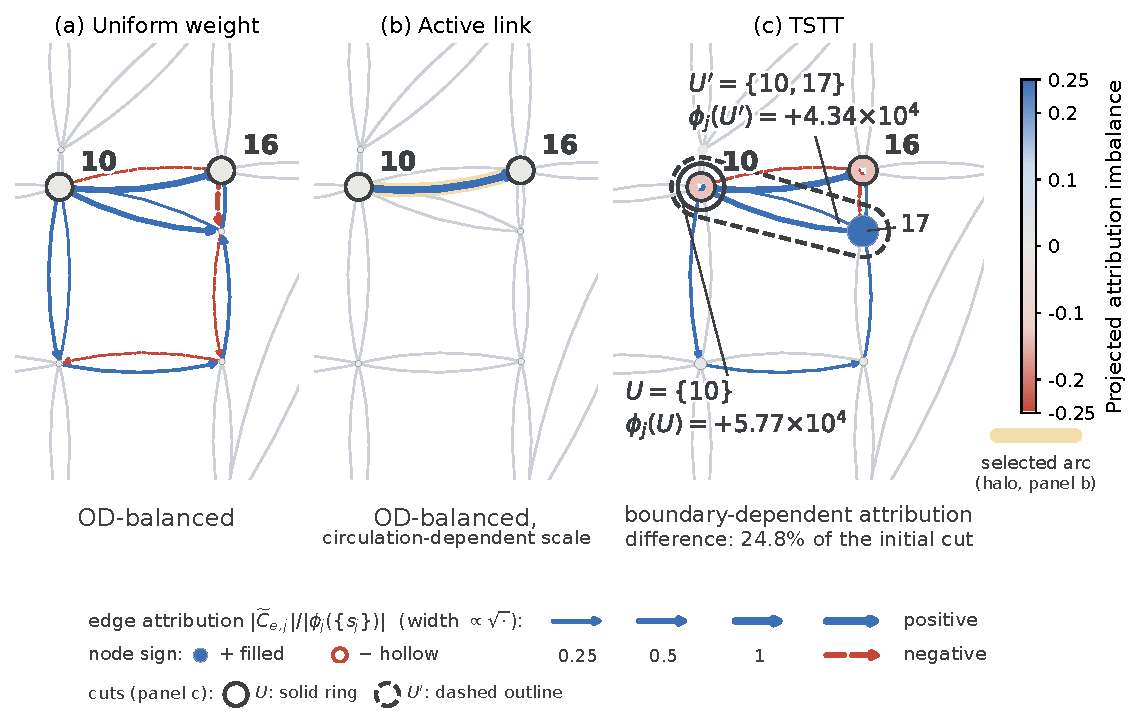
\includegraphics[width=0.9\linewidth]{../figures/fig_resp_field_v109.pdf}
\caption{OD $(10,16)$ endpoint attributions, no-background
assignment, learned
seed $0$. (a) Uniform weights give cut consistency. (b) The signed
TSTT boundary account decreases by $24.8\%$ when the boundary expands
from $\{10\}$ to $\{10,17\}$. The active-link outcome --- which
balances in the OD direction but has no response-independent scale ---
appears in Figure~\ref{fig:respfieldactive}
(Appendix~\ref{supp:accuracy}). Widths encode attribution magnitude
on the shared square-root scale; node colors show the projected
attribution imbalance $(d_j)_v$ (Eq.~\eqref{eq:endpointd}) divided by
the absolute origin-cut value.}
\label{fig:respfield}
\end{figure}

Table~\ref{tab:cutspreadperod} shows three representative queries of the eight under the three background treatments (the complete table is in Appendix~\ref{supp:additional}); rerouting produces appreciable spatial variation for every query, and connected regions retain $60.41$--$76.85\%$ of the unrestricted range across the full set. Normalizations use each setting's own origin account: for $(17,10)$, the percentage falls from $59.95\%$ under the no-background treatment to $54.77\%$ under the responsive-background treatment while the absolute spread rises from 17,607.8 to 123,202.1, approximately sevenfold.
\begin{table}[pos=htbp]
\footnotesize
\caption{TSTT cut ranges as percentages of each account's absolute
origin-cut value; three representative queries shown, complete table in
Appendix~\ref{supp:additional}. A: zero background; B: frozen background
flows; C: background demands fixed, all traffic re-equilibrated. Learned
values are five-seed medians (ranges); all SUE columns are direct
($41$ quadrature points, implicit sensitivities).}\label{tab:cutspreadperod}
\small
\begin{tabular*}{\tblwidth}{@{\extracolsep{\fill}}lccccc}
\toprule
& \multicolumn{4}{c}{Unrestricted range (\%)} & Connected (\%)\\
\cmidrule(lr){2-5}\cmidrule(lr){6-6}
OD & Learned A & SUE A & SUE B & SUE C & SUE C\\
\midrule
$(17,10)$ & $59.71$ $(58.92$--$61.23)$ & $59.95$ & $56.38$ & $54.77$ & $35.27$ \\
$(16,10)$ & $36.80$ $(36.41$--$38.40)$ & $36.86$ & $39.99$ & $166.26$ & $127.72$ \\
$(11,10)$ & $0.18$ $(0.03$--$0.27)$ & $0.0073$ & $0.79$ & $81.09$ & $48.98$ \\
\bottomrule
\end{tabular*}
\end{table}
\paragraph{Same-state response decomposition.}\label{subsec:bgsplit}
Comparing the three background treatments changes both costs and sensitivities. At each common responsive-background state, split responses into study and background parts, with $BJ_j^{\mathrm{study}}=\mu_j$ and $BJ_j^{\mathrm{bg}}=0$. Weight both by the same total-flow TSTT gradient, yielding
\begin{equation}
\widetilde C_j^{\mathrm{tot}}=\widetilde C_j^{\mathrm{study}}+\widetilde C_j^{\mathrm{bg}}.
\label{eq:bg_attribution}
\end{equation}
At node 15 for $(10,16)$, study and background divergence contributions are $-973.1$ and $49{,}103.4$. Yet on the specified expansion $\{10\}\to\{10,17\}$, the account changes only $-3361.1$ ($-1305.0$ study, $-2056.1$ background), or $1.23\%$ of the initial account. Large extremal variation can coexist with similar selected accounts. Component differences add at a fixed region pair; their separate ranges do not add in general.

\paragraph{Free-flow and congestion mechanisms.}\label{subsec:newod}
For BPR costs, $g_e'=t_{0,e}+0.75t_{0,e}(F_e/c_e)^4$. Crossing these two weight terms with the two response terms gives four additive contributions, evaluated at identical states and the same reported boundary:
\[
\phi_j(U_-)=\sum_{a\in\{\mathrm{ff,cong}\}}\sum_{b\in\{\mathrm{study,bg}\}}\phi_j^{a,b},
\qquad \phi_j^{a,b}=-\Delta q_j\int_0^1\mathbf1_{U_-}^{\top}BD_\lambda^aJ_j^b(\lambda)\,d\lambda.
\]
Table~\ref{tab:ffcong} distinguishes the mechanisms behind the sign-crossing queries of Table~\ref{tab:newod}: study congestion dominates $(1,19)$, both congestion terms are negative for $(1,15)$, and background congestion dominates $(7,12)$. The combined free-flow contribution stays positive. The decomposition is additive at a common equilibrium state and identifies the contribution of each response--weight component.
\begin{table}[pos=htbp]
\caption{Four parts of the same boundary account at the reported
$U_-$ (responsive-background six-query protocol; TSTT units; identical $41$-point
states, responses, and boundaries as Table~\ref{tab:newod}). Study
includes all six query ODs; background includes the other $522$.
Columns cross free-flow/congestion weights with study/background
responses. Entries are rounded independently.}\label{tab:ffcong}
\small
\begin{tabular*}{\tblwidth}{@{\extracolsep{\fill}}lrrrrr}
\toprule
OD & Free-flow study & Free-flow background & Congestion study & Congestion background & Total\\
\midrule
$(1,19)$ & $-361.3$ & $+759.0$ & $-17{,}357.9$ & $+3{,}458.6$ & $-13{,}501.6$ \\
$(1,15)$ & $+1{,}541.8$ & $+333.8$ & $-6{,}537.4$ & $-3{,}624.2$ & $-8{,}286.0$ \\
$(7,12)$ & $+3{,}897.0$ & $-1{,}311.1$ & $+125.5$ & $-20{,}327.6$ & $-17{,}616.2$ \\
\bottomrule
\end{tabular*}
\end{table}
The sign pattern itself is a spatial property, not a magnitude artefact. Negative accounts occupy $17.8\%$, $2.5\%$ and $7.3\%$ of the 14,477, 15,191 and 16,943 connected regions of the three sign-crossing queries. For $(1,19)$, the connected minimum $-13{,}501.6$ is attained on a 13-node region, whereas a 13-node free-flow neighbourhood has account $+10{,}756.0$: region size alone does not determine the account. At the minimizing boundary, outgoing attributions sum to $7{,}867.3$ and incoming attributions to $21{,}368.8$, so the signed crossing-link account is negative while $C_j=50{,}097.7>0$; Figure~\ref{fig:negmech} maps all 26 crossing links. Figure~\ref{fig:screenlines} shows the same contrast on two straight screenlines of the prespecified geometric family: the minimum and maximum screenline accounts of $(1,19)$ have opposite signs under one positive network-wide contribution.
\begin{figure}[pos=tb]
\centering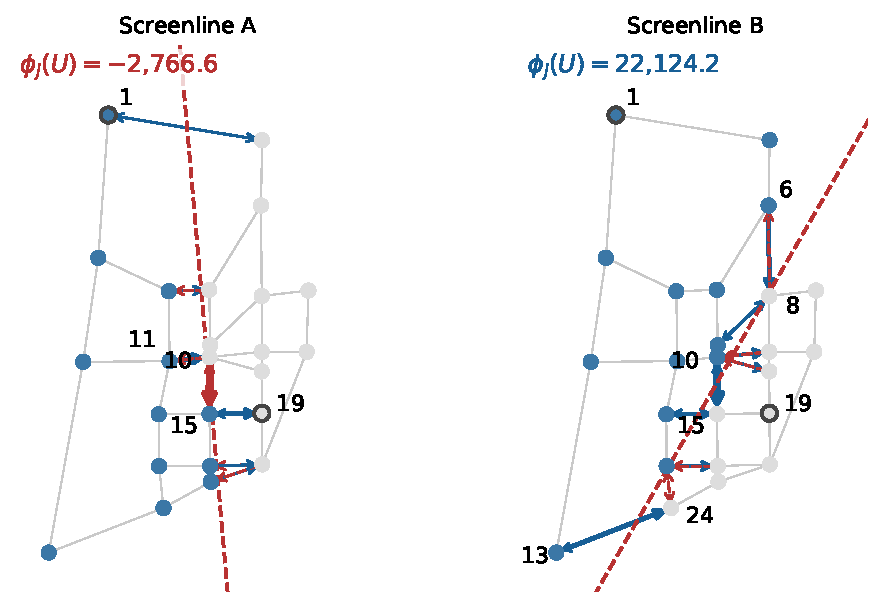
\includegraphics[width=0.66\linewidth]{../figures/fig_screenlines_v109.pdf}
\caption{Contrasting screenline accounts for the same positive OD
contribution. Two straight screenlines for OD $(1,19)$ under the
responsive-background assignment. Blue nodes belong to $U$; grey nodes
are outside; dashed lines separate the two sides. Node $1$ is inside
and node $19$ outside in both panels. The two lines have different
normal directions, so they are labelled Screenline~A (left) and
Screenline~B (right); the crossing progress of each with the straight
origin--destination segment is $0.61$ and $0.78$, an ordering of the
crossing positions that does not by itself make the two enclosed
regions nested. The two accounts have opposite signs while the
network-wide contribution is positive; arrows encode the signed
crossing contributions (solid blue = positive, dashed red = negative,
width = magnitude). Principal crossing contributions, Screenline~A:
$10\to15$ $-9195.2$, $11\to10$ $+3169.6$, $15\to19$ $+2689.9$;
Screenline~B: $10\to15$ $+9195.2$, $13\to24$ $+3602.1$, $6\to8$
$+3508.8$ (TSTT units). The lines are the minimum and maximum of the
prespecified geometric family; the complete irregular connected minimum
and its crossing-link decomposition appear in
Figure~\ref{fig:negmech}.}
\label{fig:screenlines}\end{figure}
The straight-screenline family uses 36 directions at $5^\circ$ intervals, gaps between node projections, two-sided connectivity and duplicate removal; construction is independent of attribution. It contains 23--152 distinct regions per query. The $(1,19)$ and $(7,12)$ negative minima occur on 2/152 and 10/148 screenlines. Origin-centred hop and free-flow neighbourhoods remain positive but can differ in magnitude by factors 8.9, 9.0 and 3.4 for the three sign-crossing queries (Appendix~\ref{supp:newodaccuracy}). Sign stability and common-value accuracy are distinct properties.

\paragraph{Stability under alternative attribution paths.}\label{subsec:pathrobust}
With several ODs changing jointly, the per-query attribution columns
depend on the demand path; the columns are defined here under the
straight-line transition, and this paragraph quantifies that
dependence. Twenty-two piecewise-linear alternatives --- the six study
ODs changing one at a time, in canonical order, reverse order, and
twenty fixed-seed random permutations --- are compared with the
straight line on the responsive-background protocol, with identical endpoints,
solver tolerance, quadrature and boundary family, and with the
mechanism decomposition evaluated at the same fixed regions $U_-$; the
total outcome change is path independent and reproduces to
$1.5\times10^{-7}$ relative on every order.

The spatial conclusions are order-insensitive: system contributions move by at most
$3.4\%$, every query's sign-crossing status over the family is
identical on all 22 orders, the normalized common-summary errors shift
by at most $0.2$ percentage points, and the dominant mechanism at $U_-$
is unchanged on every order. The profile deviations themselves are
bounded (medians $0.3\%$--$4.5\%$, maxima $0.3\%$--$4.7\%$ of the
largest straight-line account), so the reported profiles are
path-specific in their fine structure but not in their traffic
interpretation. The complete per-order comparison appears in
Table~\ref{tab:pathrobust} (Appendix~\ref{supp:pathrobust}).
